\section{Motivation and experimental context}
In many systems, cortical flows are driven not by continuous contraction of active material, but by repeated rounds of pulsatile contraction.  While it was once believed that these pulsatile behaviors could be an emergent property of actomyosin contractility itself, it is now more probably suspected that 

It is still unclear why so many systems exhibit this type of behavior, it is nonetheless important to understand the origins of these behaviors and what differences may arise due to their presence or absence in a contractile system.  Therefore, we have begun exploring how to model both the upstream regulators that govern contractile systems as well as the downstream effects of coupling these to regulators to contractile flows themselves.

The majority of our data comes from the work of Francois Robin and Jon Michaux (cite).  They have shown that upstream of both actin and myosin is a separate pulsatile biochemical circuit consisting of a combination of positive and negative feedback between a pair of proteins called Rho and RGA as depicted in Figure \ref{fig:pulse_diag}.  For more information on the biochemistry of this circuit please see their paper (cite again).  

\begin{figure}[h!]
\centering
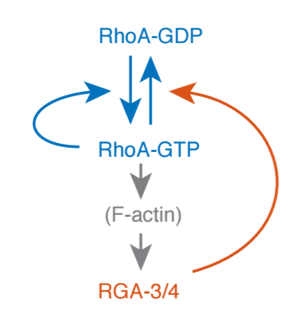
\includegraphics[width=0.5\hsize]{pulse/diagram.png}
\caption{\label{fig:pulse_diag}  Proposed reaction pathway for Rho excitability.}
\end{figure}

To explain the dynamics we attempted to build ordinary differential equation models of local variation in active Rho and RGA concentrations.  We found that many models are effectively equivalent at producing the qualitative results.  However, all of our models were fairly bad at producing robust pulsatile behavior once the models were constrained by parameter fitting to the data. 

\section{A model for pulsatile actomyosin accumulation in \textit{C. elegans} }

My first attempt at modeling involved a fair

I defined $\rho$ as the concentration of Rho and $r$ as the concentration of RGA, and generated association, dissociation and feedback parameters for the model. 

\begin{equation}
\label{eqn:rho_1}
	\frac{d\rho}{dt} = k_{on}^\rho \left( 1+k_{on}^{\rho\rho} \frac{\rho^n}{\rho_0^n +\rho^n} \right ) - (k_{off}^\rho + k_{off}^{\rho r} r) p
\end{equation}

\begin{equation}
\label{eqn:rga_1}
	\frac{dr}{dt} = k_{on}^{r \rho}\rho - k_{off}^r r 
\end{equation}

Next we can nondimensionalize the equation with $q=\rho/\rho_0$, $s=k_{off}^{\rho r}/k_{off}^r r$, and $\tau=k_{off}^r t$, and rename parameters for simplicity.

\begin{equation}
	\frac{dq}{d\tau} = k_q \left( 1+k_{qq} \frac{q^n}{1 +q^n} \right ) - (k_{off} + s) q
\end{equation}

\begin{equation}
	\frac{ds}{d\tau} = k_s q - s
\end{equation}

The null-clines are 

\begin{equation}
	s_q =\frac{k_q}{q} \left( 1+k_{qq} \frac{q^n}{1 +q^n} \right ) - k_{off} 
\end{equation}

\begin{equation}
	s_s = k_s q
\end{equation}

\begin{figure}[h!]
\centering
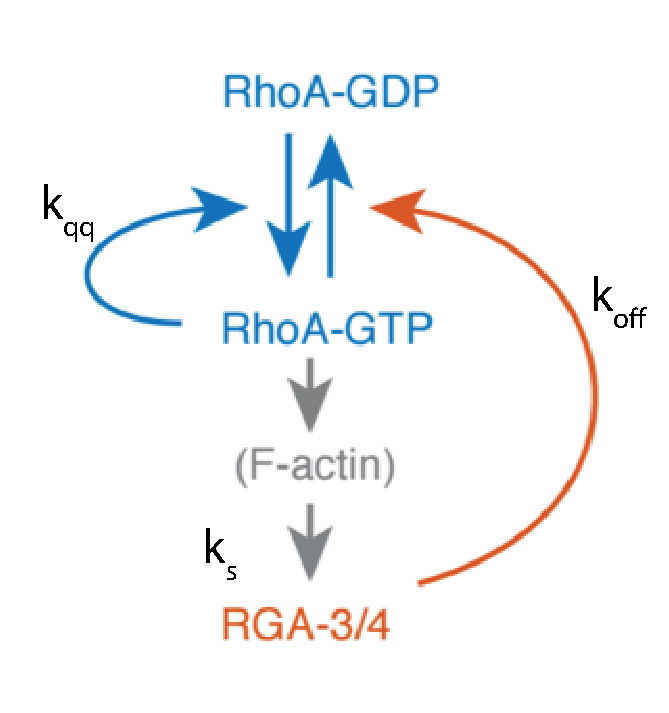
\includegraphics[width=0.5\hsize]{pulse/diagram_eq.eps}
\caption{\label{fig:pulse_diag}  Reaction pathway with labels for coefficients associated with feedback stregths.}
\end{figure}

\subsection{Analyzing parameter space of the model}

\begin{figure}[h!]
\centering
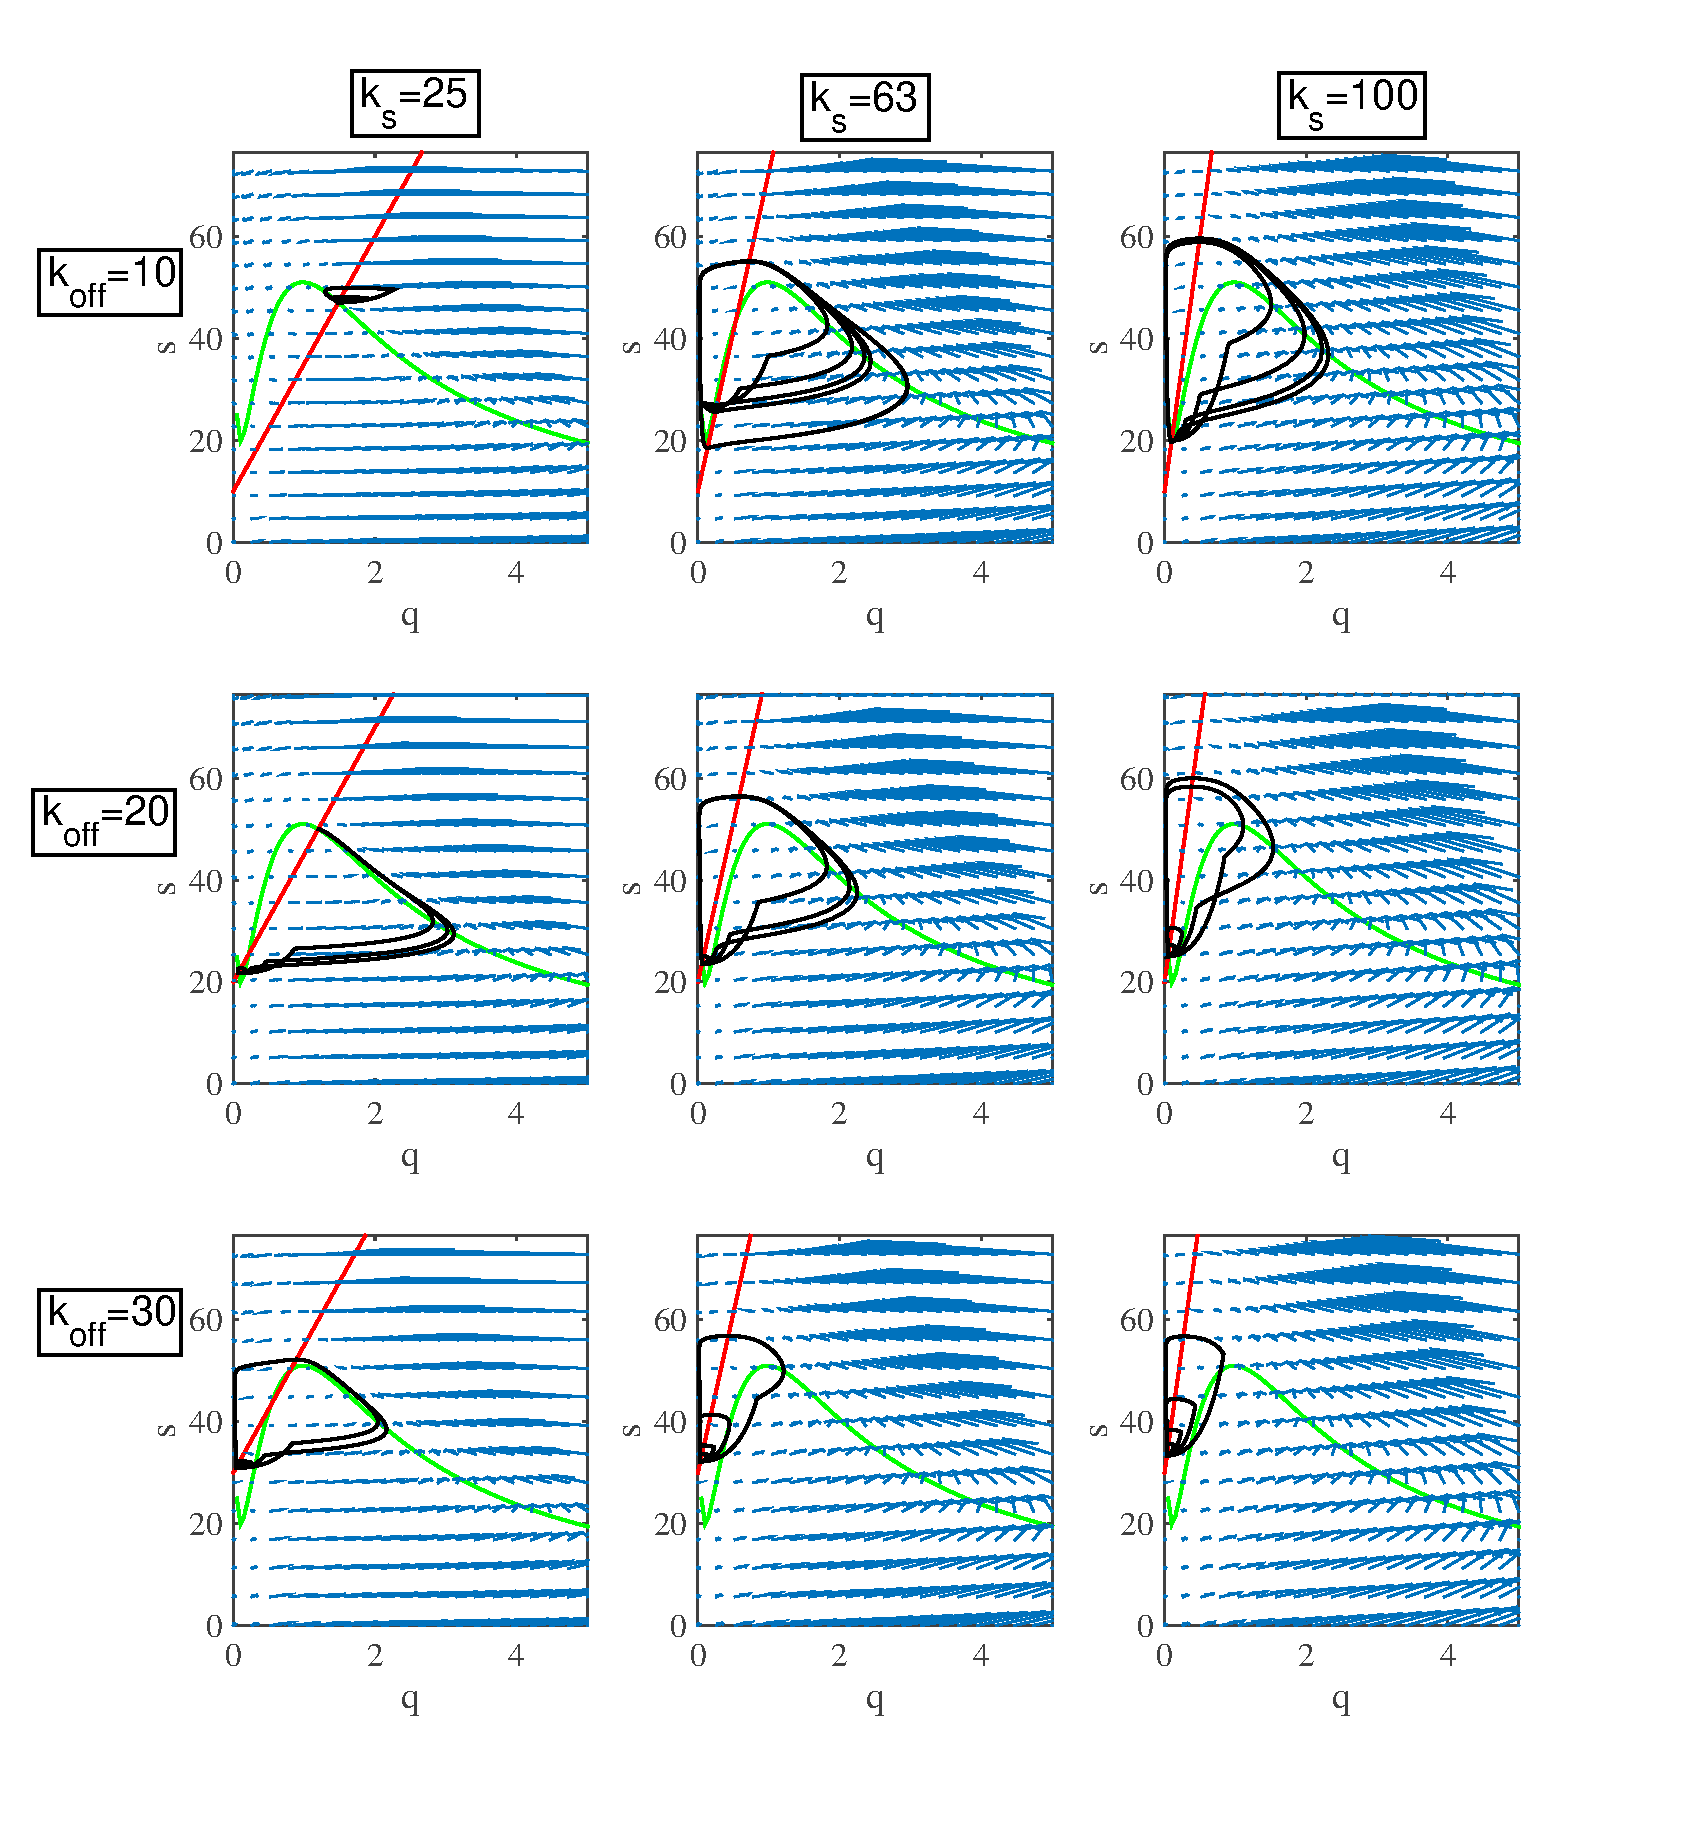
\includegraphics[width=\hsize]{pulse/phase_tester.eps}
\caption{\label{fig:pulse_fit}  Phase diagram of for $k_q=1$ and $k_qq=100$.}
\end{figure}

\begin{figure}[h!]
\centering
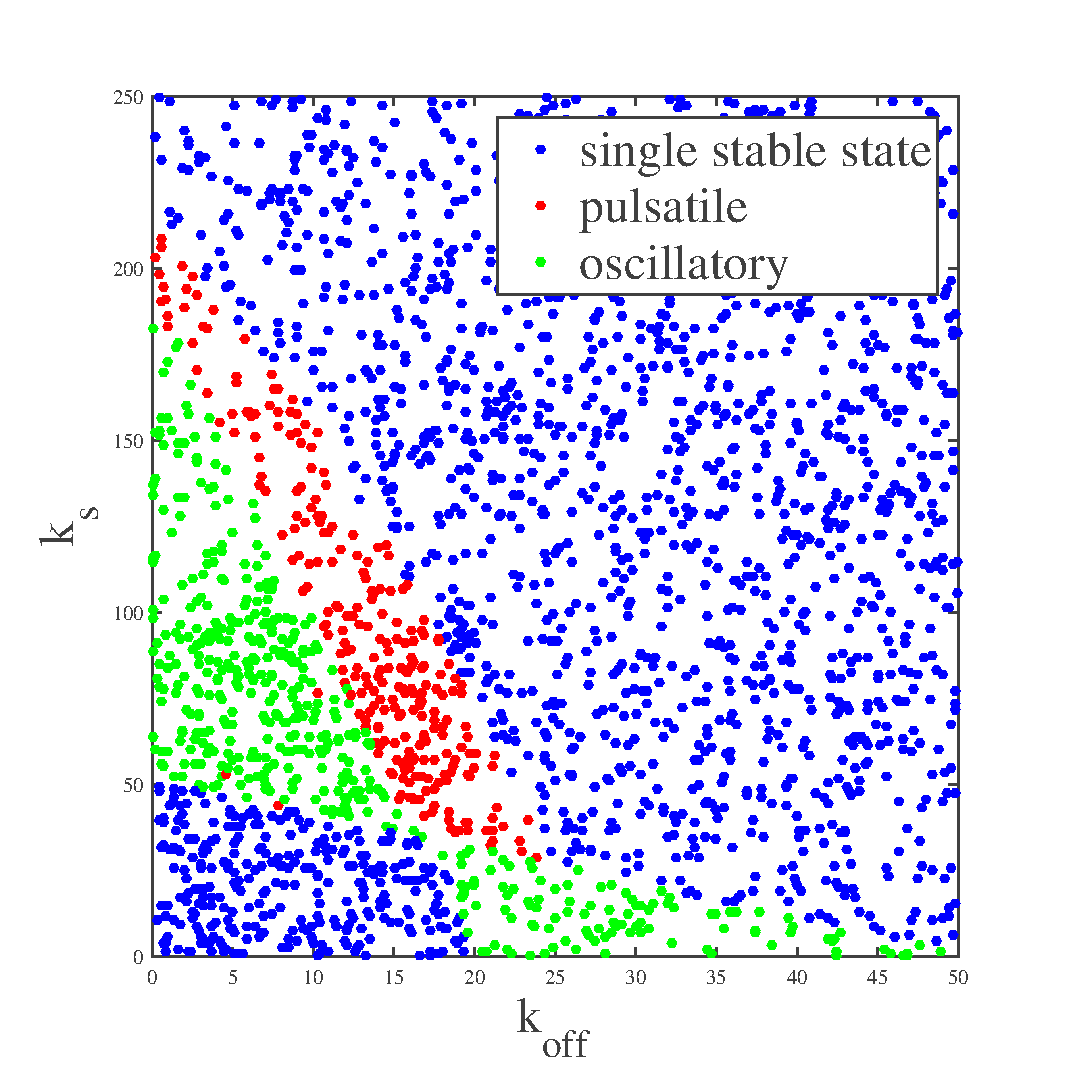
\includegraphics[width=\hsize]{pulse/k_phase.eps}
\caption{\label{fig:pulse_fit}  Phase diagram of for $k_q=1$ and $k_qq=100$.}
\end{figure}

\begin{figure}[h!]
\centering
\includegraphics[width=\hsize]{pulse/randomized_simulation.eps}
\caption{\label{fig:pulse_fit}  Phase diagram of for $k_q=1$ and $k_qq=100$.}
\end{figure}

\section{Simplified model and data fitting}

Although 

\begin{equation}
	\frac{dq}{d\tau} =\alpha \frac{q^n}{1 +q^n} - s q^k
\end{equation}

\begin{equation}
	\frac{ds}{d\tau} = \beta q^{(m-k)} - s
\end{equation}

These equations resulted in a family of models with different levels of feedback, depending on the values of $n$, $m$, and $k$.  I fit models with a variety of exponents and found that any model with $k\approx0$, $n>1$, and $m\approx2$ gave the best overall agreement with the greatest robustness.  

\subsection{Fitting techniques}
I used two different methods to fit the Rho and RGA data to determine the most appropriate model parameters.  The first required subsecting the data to fit only to regions where some parameters were presumable close to constant.  For example, as long as RGA concentration remained relatively small, the .


\begin{figure}[h!]
\centering
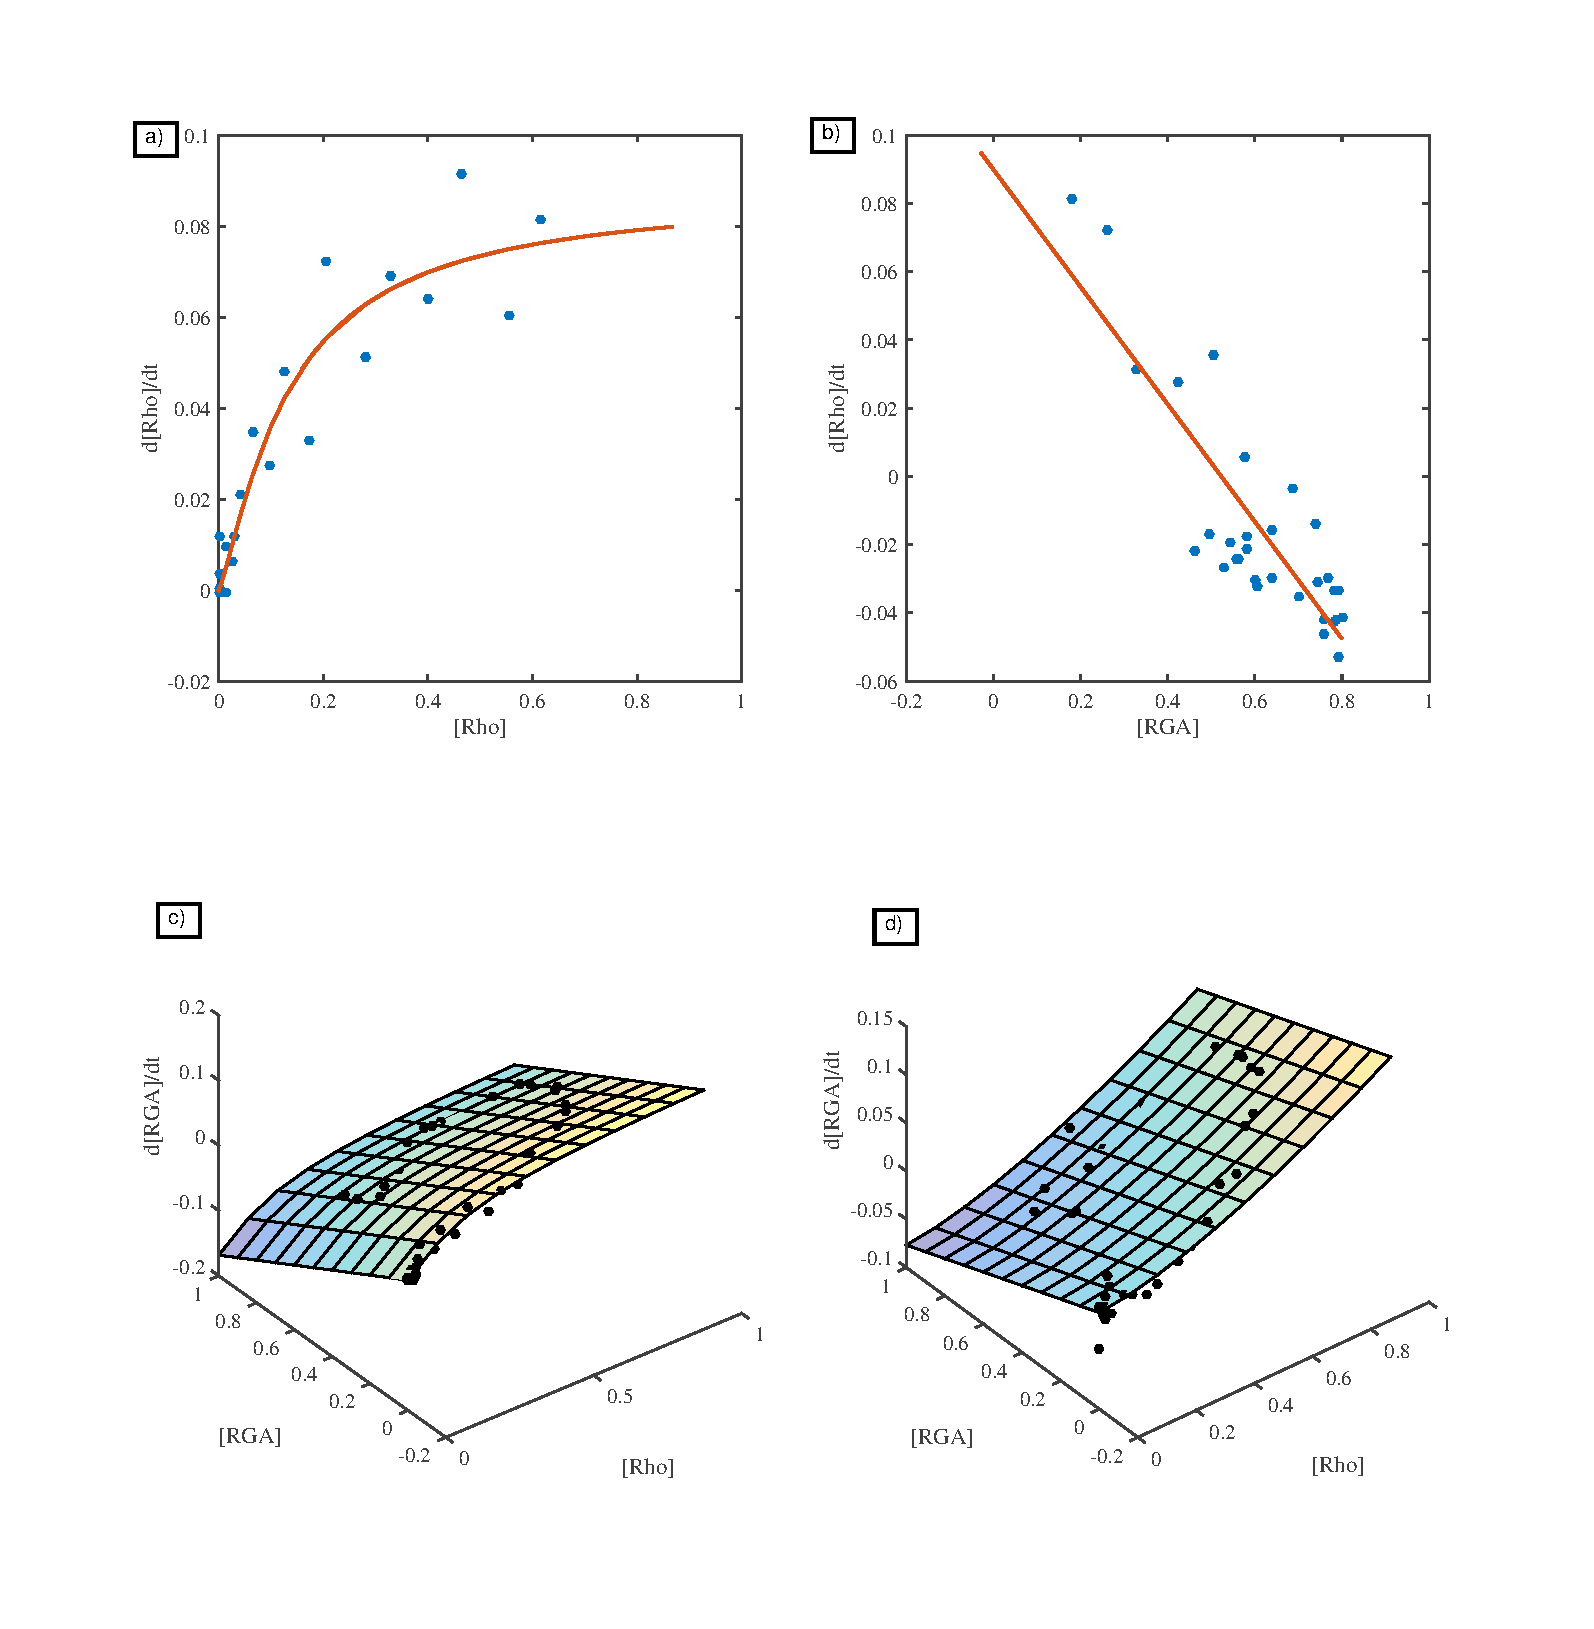
\includegraphics[width=\hsize]{pulse/fitting_plot.eps}
\caption{\label{fig:pulse_fit}  Multiple methods of fitting.}
\end{figure}

\begin{figure}[h!]
\centering
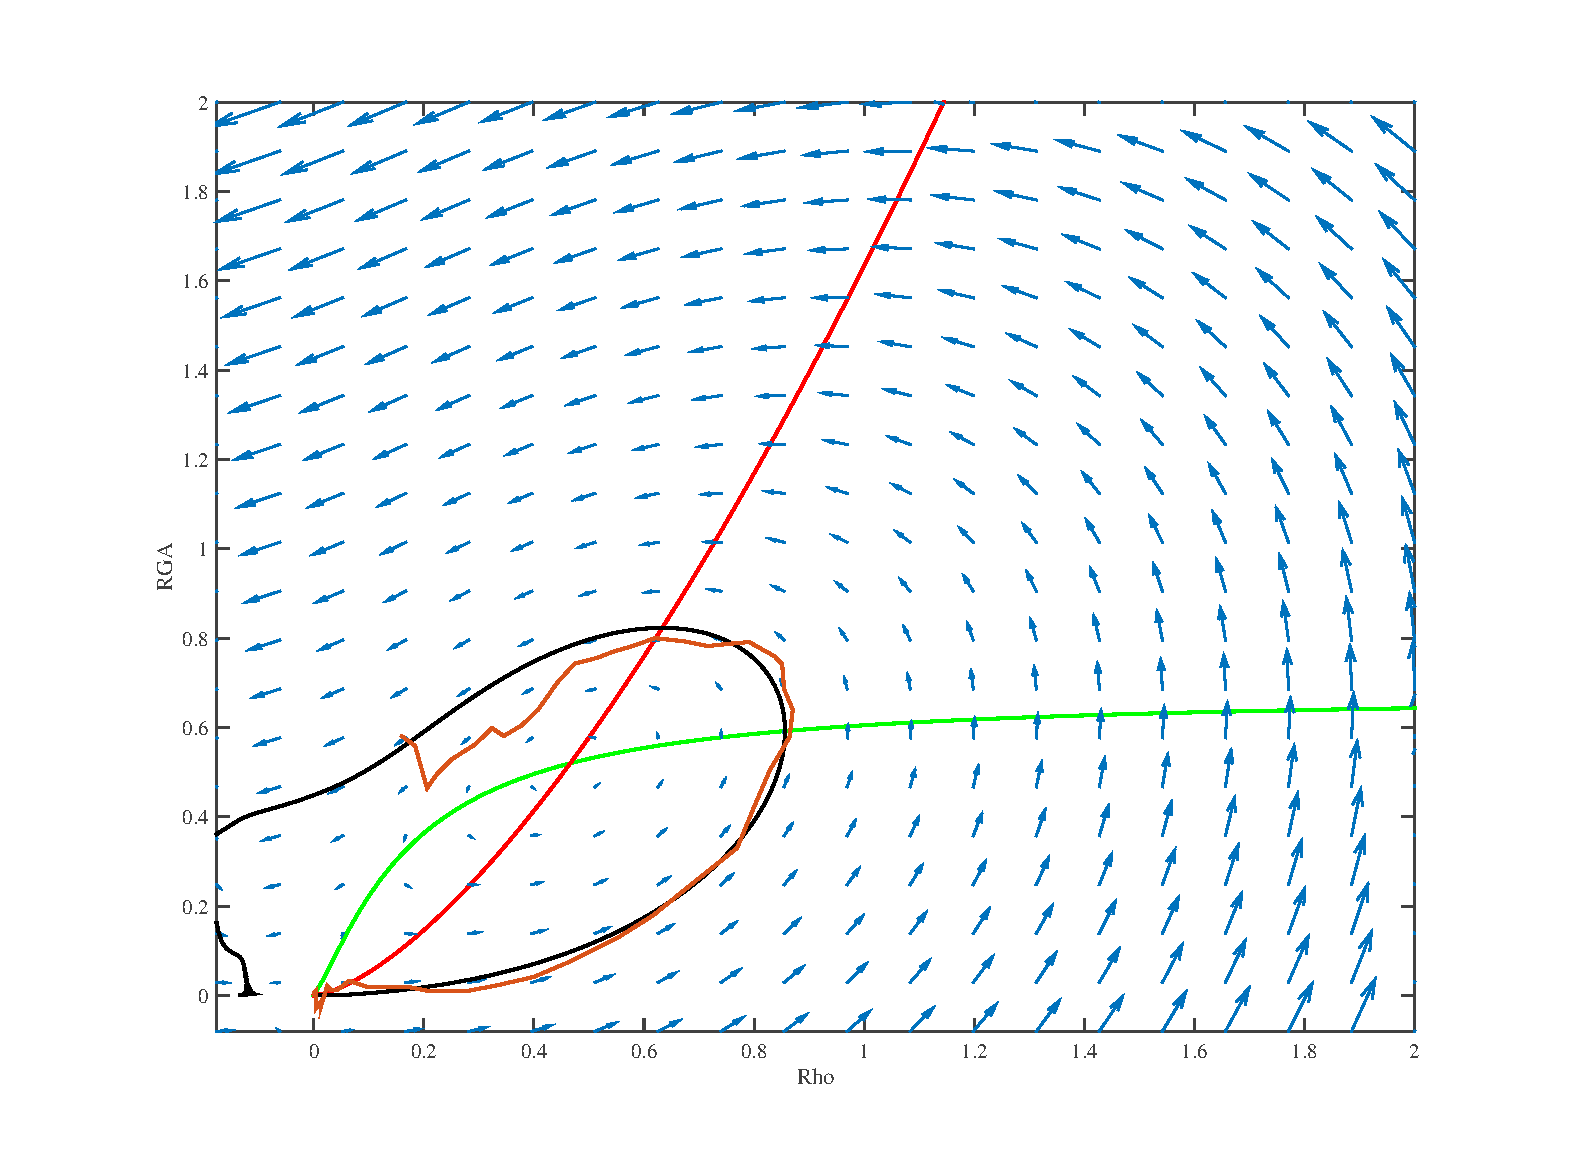
\includegraphics[width=\hsize]{pulse/simple_model_fit_phase.eps}
\caption{\label{fig:pulse_fit_phase}  Simulation results and fitted for phase diagram.}
\end{figure}

\begin{figure}[h!]
\centering
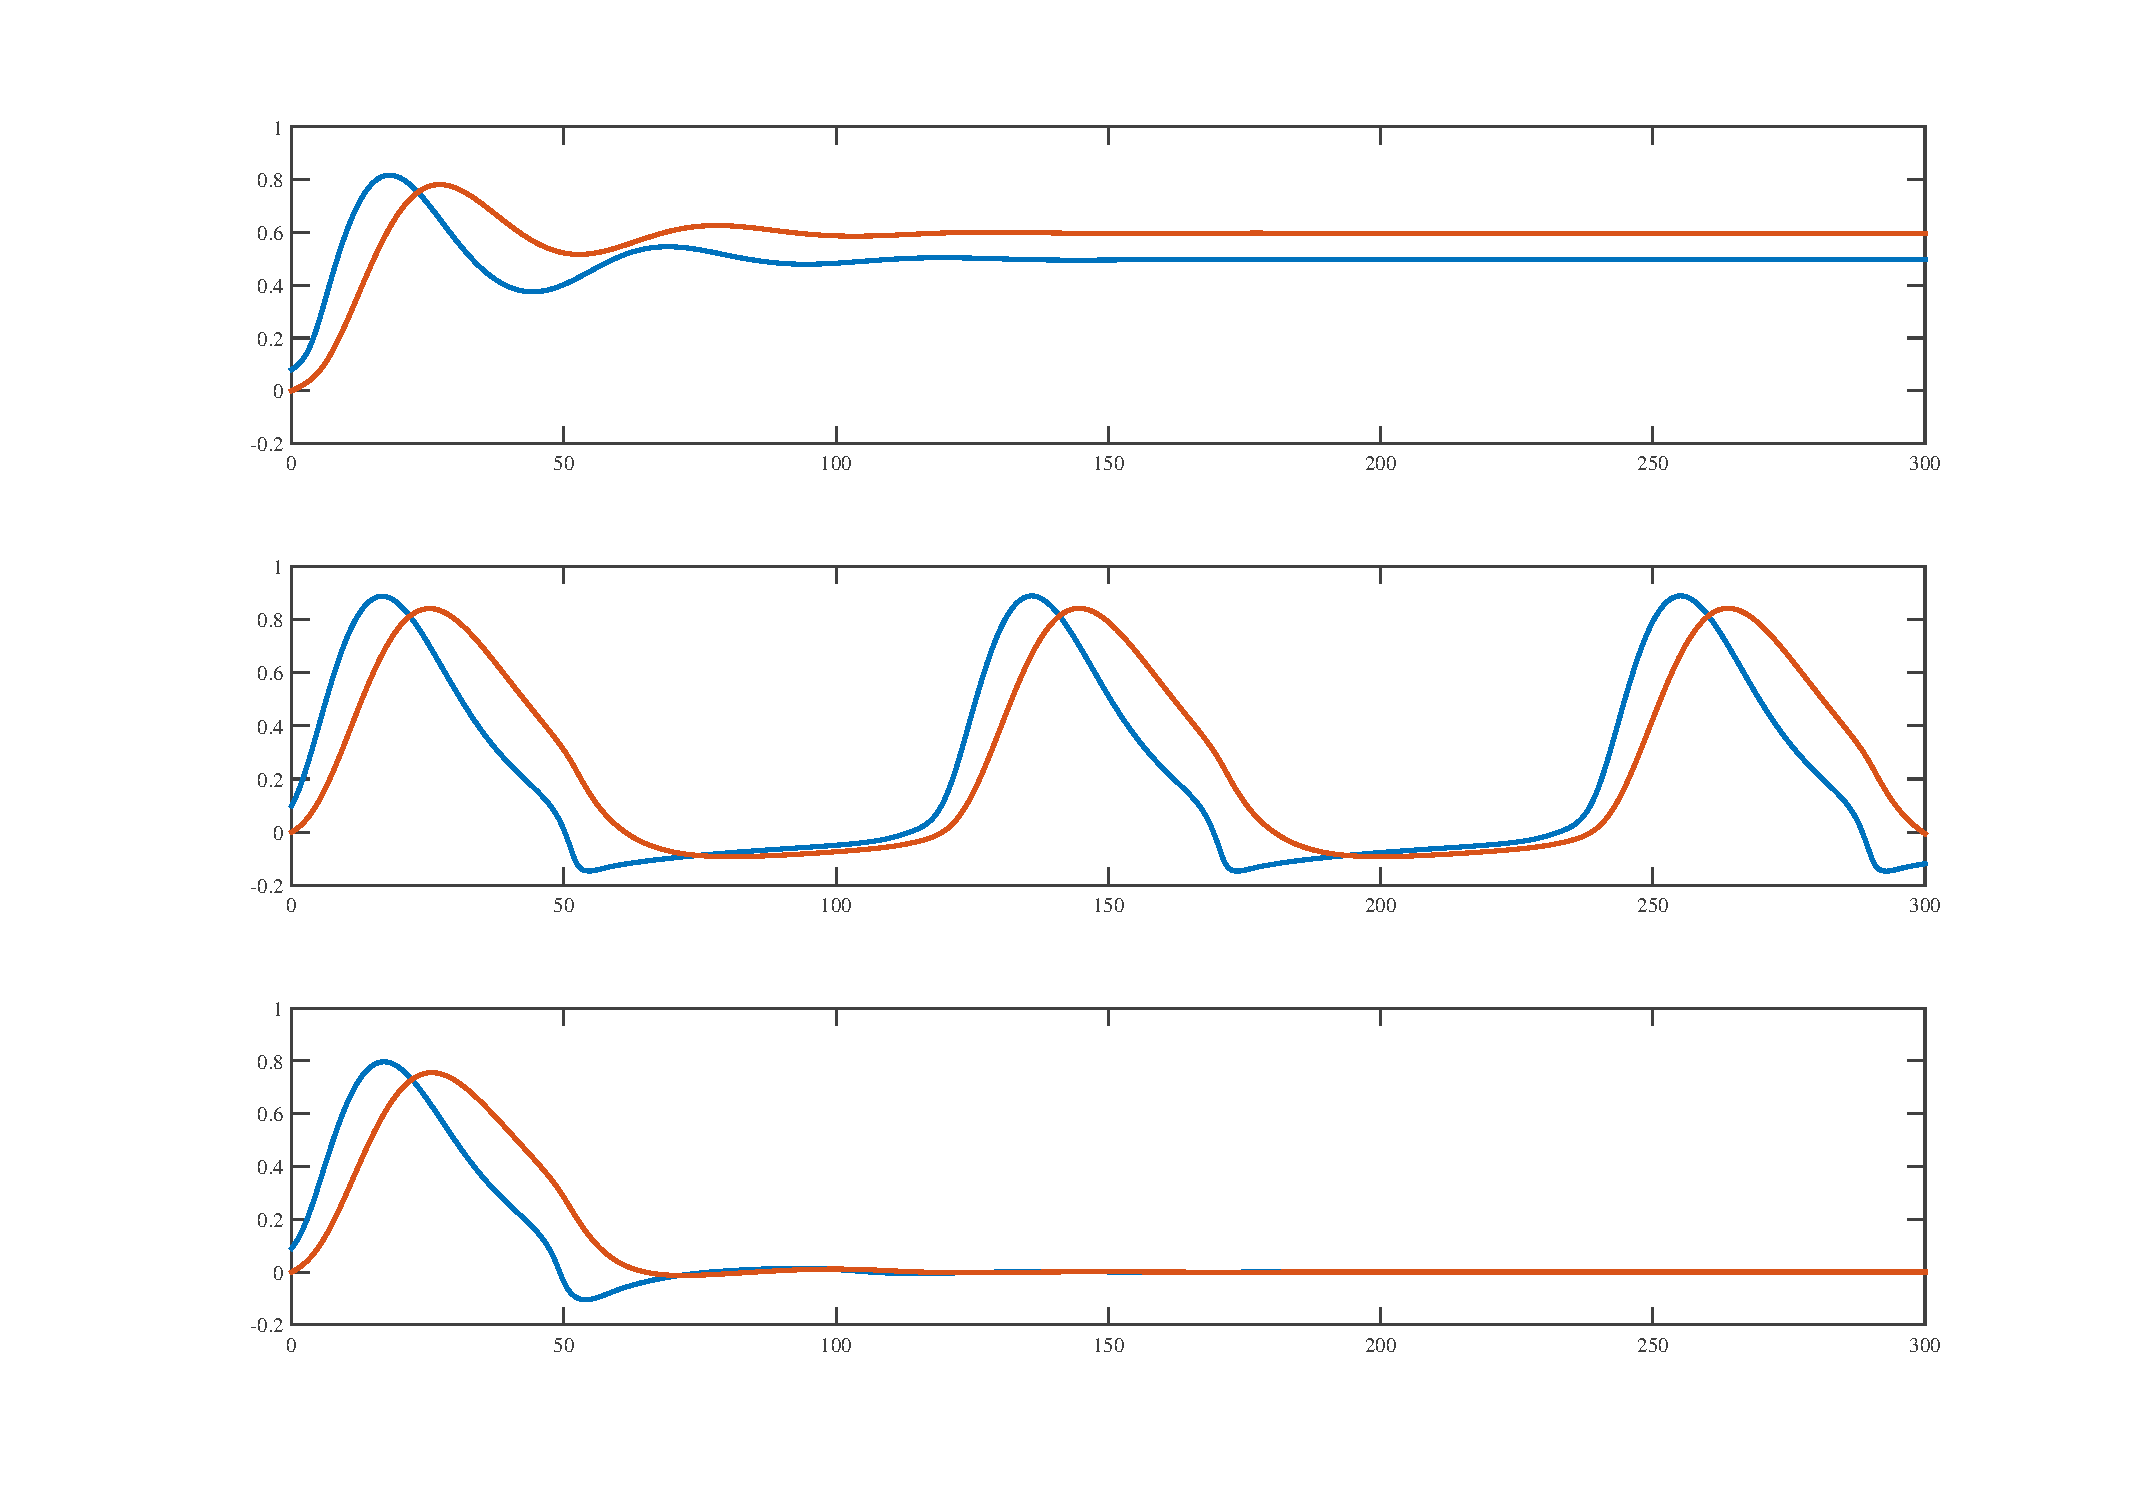
\includegraphics[width=\hsize]{pulse/model_compare.eps}
\caption{\label{fig:pulse_fit_phase}  Simulation results and fitted for phase diagram.}
\end{figure}

\begin{figure}[h!]
\centering
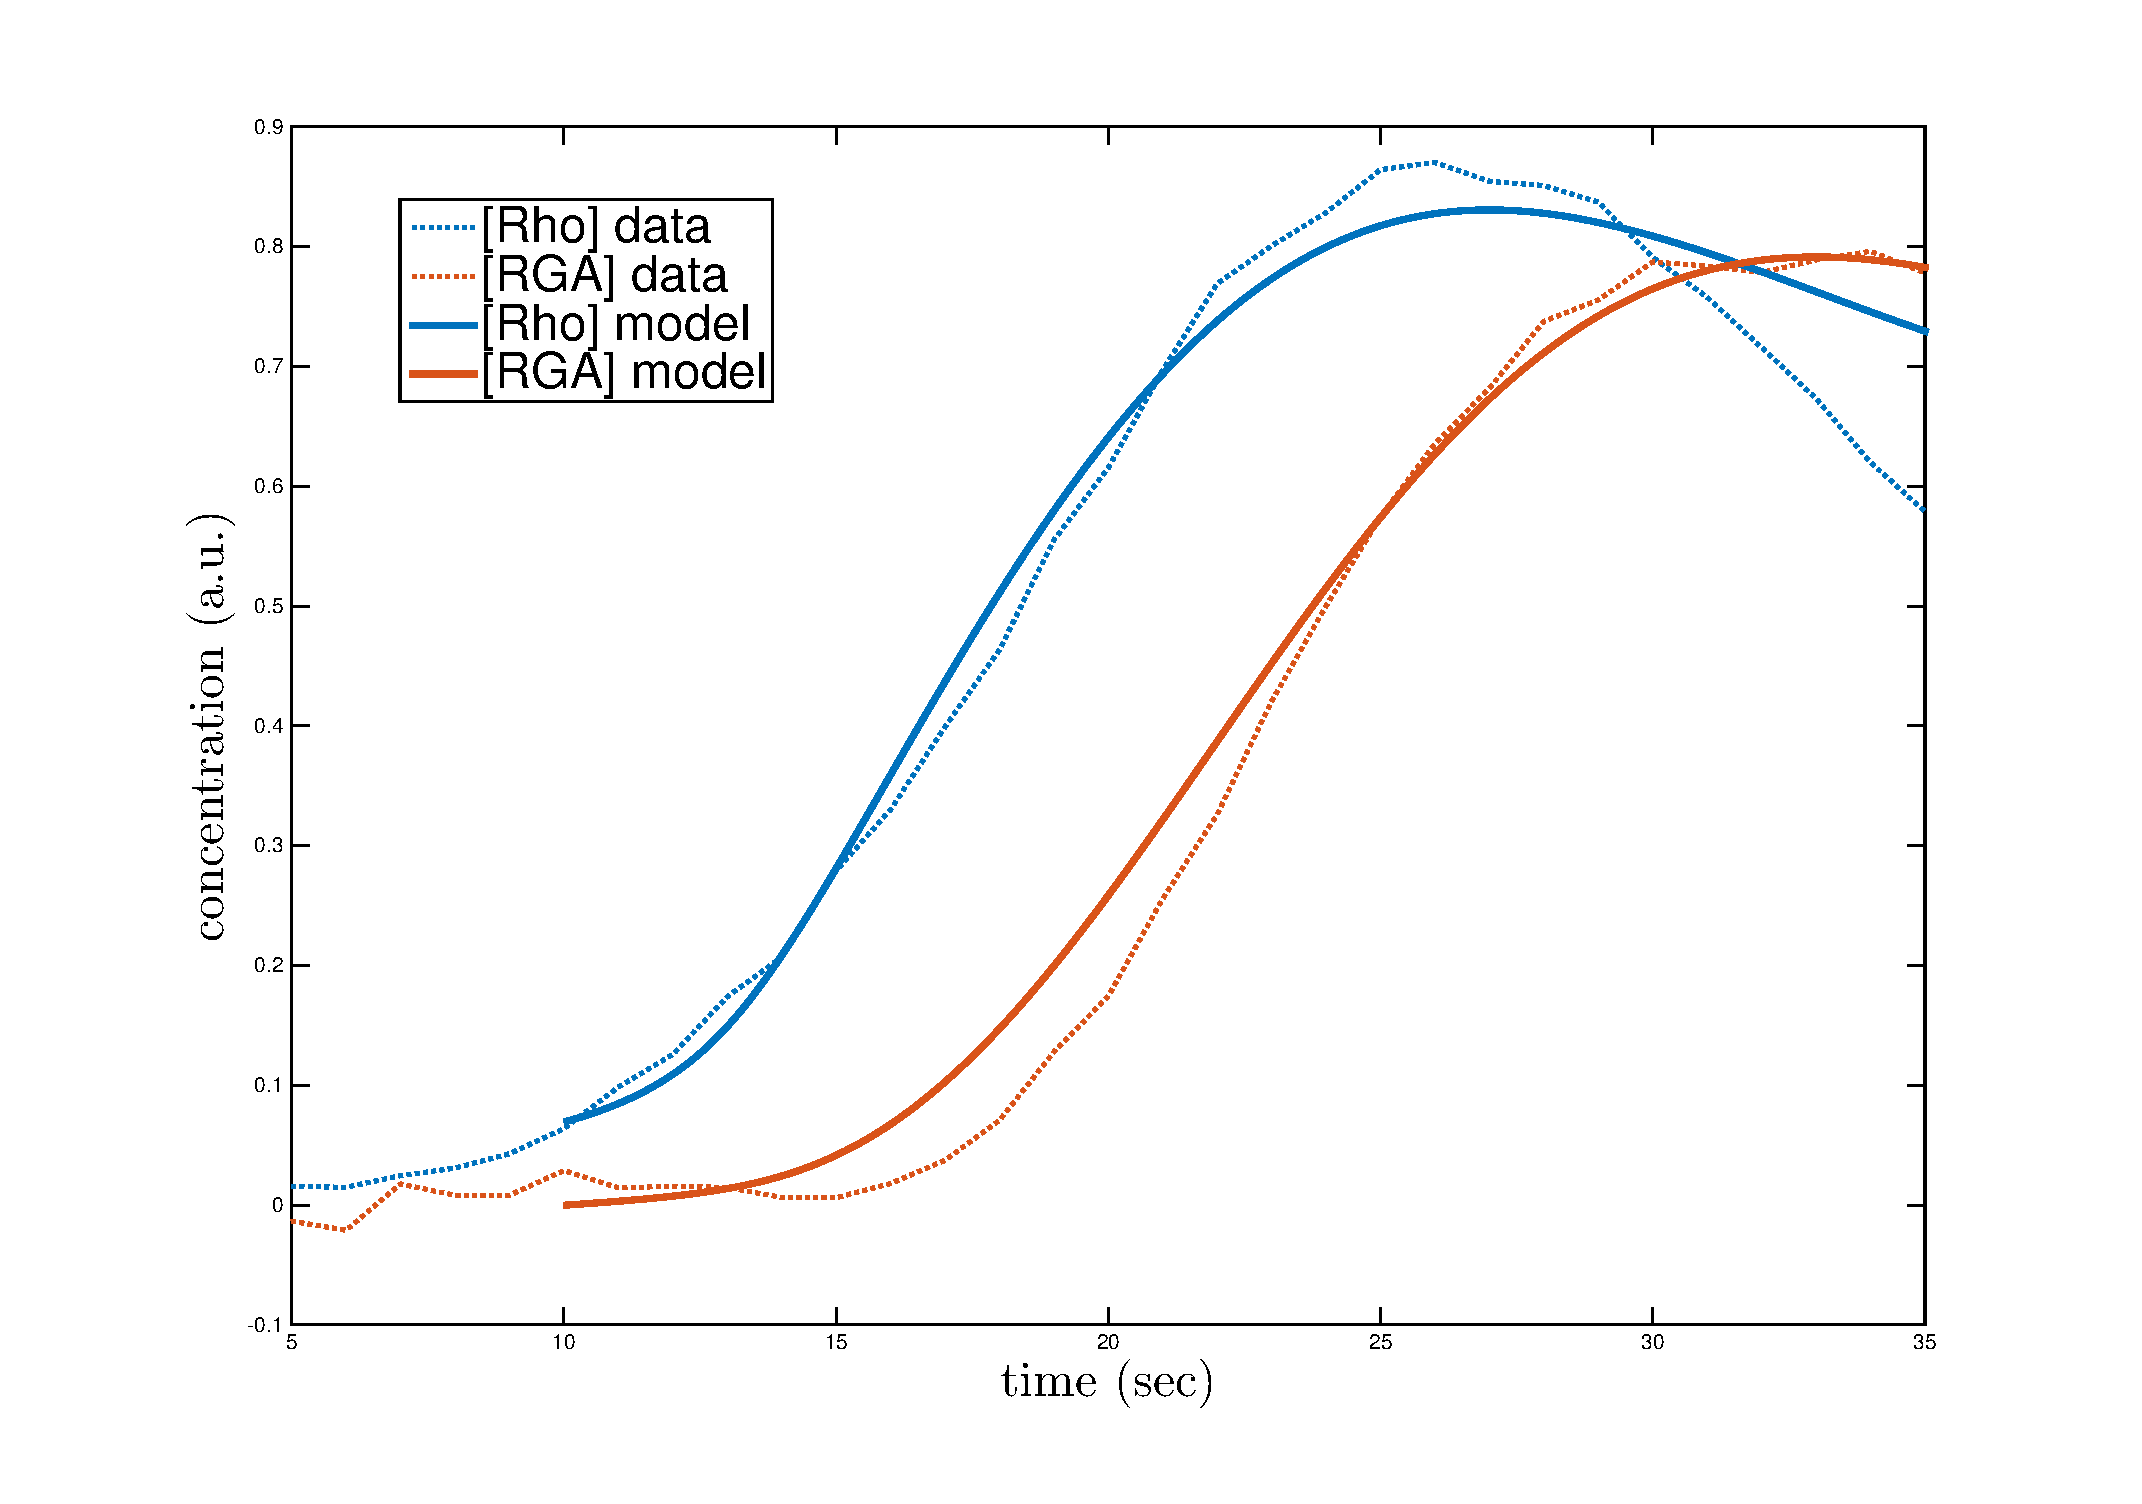
\includegraphics[width=\hsize]{pulse/model_profile.eps}
\caption{\label{fig:pulse_fit_phase}  Simulation results and fitted for phase diagram.}
\end{figure}




\section{Conclusion}
\begin{figure}[h!]
\centering
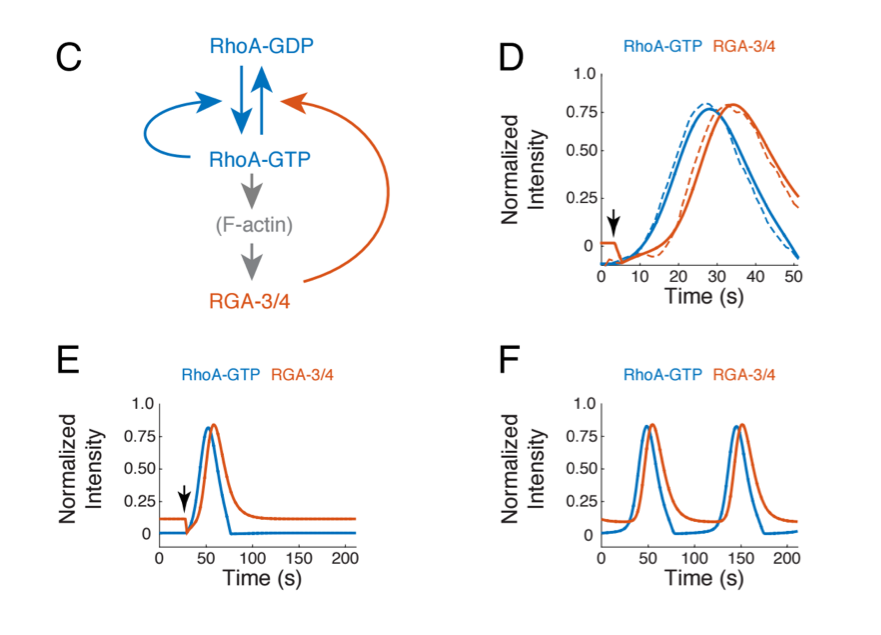
\includegraphics[width=\hsize]{pulse/final_fig.png}
\caption{\label{fig:pulse_final}  Final figure as it appears in Robin et al.}
\end{figure}
Ultimately, a model similar to \ref{eqn:rho_1} and \ref{eqn:rga_1} was utilized in the final paper in combination with at the 2D fitting routine outlined in Figure \ref{fig:pulse_fit}c,d.   In short, all models performed equally well (or poorly depending on perspective) at describing the qualitative features of the data, but none were very effective at generating a quantitative match.    We believe this is indicative of the need to perhaps extend to incorporating spatial effects in driving the dynamics of active material pulses.

Based on the theoretical results of [bois and the other one], we attempted to incorporate our upstream regulatory model into a 1D active fluid.  

